
\section{Nouniform Amplitude}
\subsection{要求}
\noindent 比较几种不同幅度激励的等间距($\lambda/4$)10元边射阵方向图.并分别计算他们的第一旁瓣电平和HPBW. 


1.均匀分布  $a_1=a_2=a_3=a_4=a_5=1$

2.二项式分布 $a_1=126, a_2=84, a_3=36, a_4=9, a_5=1$

3. Dolph-Tschebyscheff分布$a_1=2.798, a_2=2.496, a_3=1.974, a_4=1.357, a_5=1$
\\

\noindent 选做:

1.根据第4题1中的计算的10元均匀分布情形,用编程数据计算HPBW和D0,并与Tschebyscheff阵的经验预估值(6.8.3-C部分)比较

2.若选单元为沿z轴放置的元天线,根据图乘法画出总方向图
\\
\noindent 提示:电偶极子元天线方向图(垂直于z轴放置 )
\begin{equation}
EF=E_\theta=j\eta\dfrac{kI_0le^{-jkr}}{4\pi r}\cos\theta
\end{equation}


\subsection{原理及推导}
对于N元阵,其阵因子
\begin{equation}
AF_{2M}(even)=\sum_{n=1}^{M}a_n\cos\left[\left(2n-1\right)u\right].
\end{equation}
\begin{equation}
AF_{2M}(odd)=\sum_{n=1}^{M+1}a_n\cos\left[2\left(n-1\right)u\right].
\end{equation}
其中
\begin{equation}
u=\frac{\pi d}{\lambda}\cos\theta
\end{equation}

考虑单元因子的情况下, 根据图乘法, $TF=AF\times EF$,编程也很容易计算.  

\subsection{结果与分析}
\subsubsection{不同幅度激励的等间距10元边射阵}

\paragraph{HPBW}

如表\ref{tab:hpbw}所示, 发现二项式激励的HPBW和等幅激励相比变胖了很多,而切比雪夫激励的HPBW则变化很小,有良好的方向性,可以认为是最优的激励方式.
\begin{table}[!ht]
	\centering
	\begin{tabular}{c|ccc}
		\toprule
		激励方式&等幅激励&二项式激励&切比雪夫激励\\
		\midrule
		HPBW /$^\circ$&24.3360  &48.8160 &  29.5200\\
		\bottomrule
	\end{tabular}
	\caption{不同激励方式的HPBW} \label{tab:hpbw}
\end{table}

\paragraph{第一旁瓣电平(功率)}
如图\ref{fig:LobeValue}所示,二项式激励不存在旁瓣,而切比雪夫激励的旁瓣电平远远小于等幅激励的第一旁瓣电平.

\textit{注:图中标注的点,并非是第一旁瓣电平,而是第一旁瓣的归一化辐射功率(非dB),二者的物理本质是相同的,故不做区分. }
\begin{figure}[!ht]
	\centering
	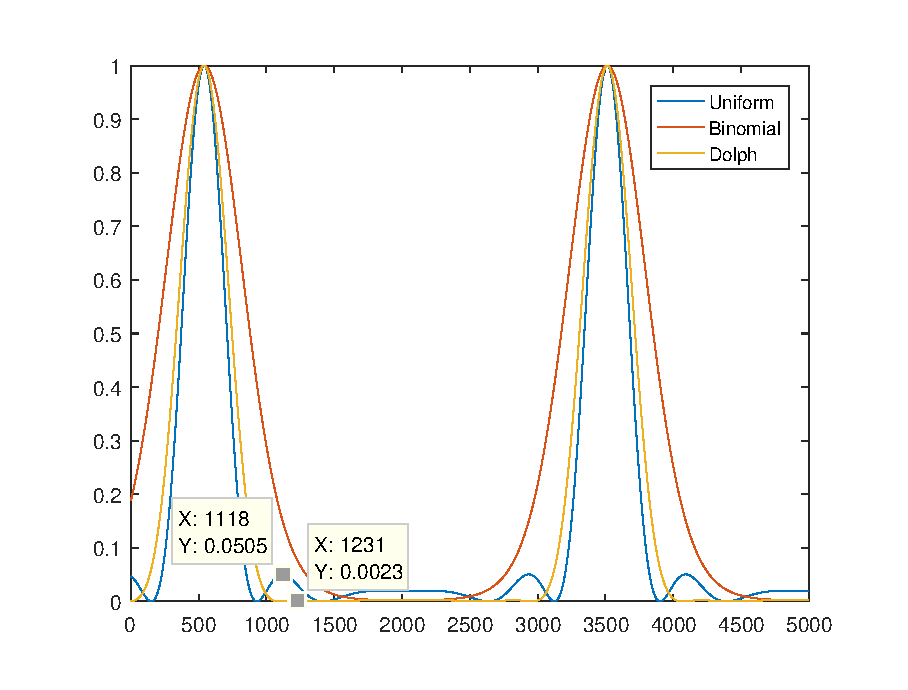
\includegraphics[width=10cm]{TenEle_without_EF_lobeValue.eps}
	\caption{第一旁瓣功率} \label{fig:LobeValue}
\end{figure}


\paragraph{方向图}


根据图\ref{fig:10elenoEF}所示,放大观察如图\ref{fig:10elenoEF_fangda}.

容易发现, 二项式分布的激励,理论上没有任何旁瓣,但是HPBW明显增加.而Dolph-Tschebyscheff分布的激励,其旁瓣电平很小,而且HPBW也很窄,可以认为是最优分布. 
\begin{figure}[!ht]
	\begin{minipage}[t]{0.35\linewidth}
		\centering
		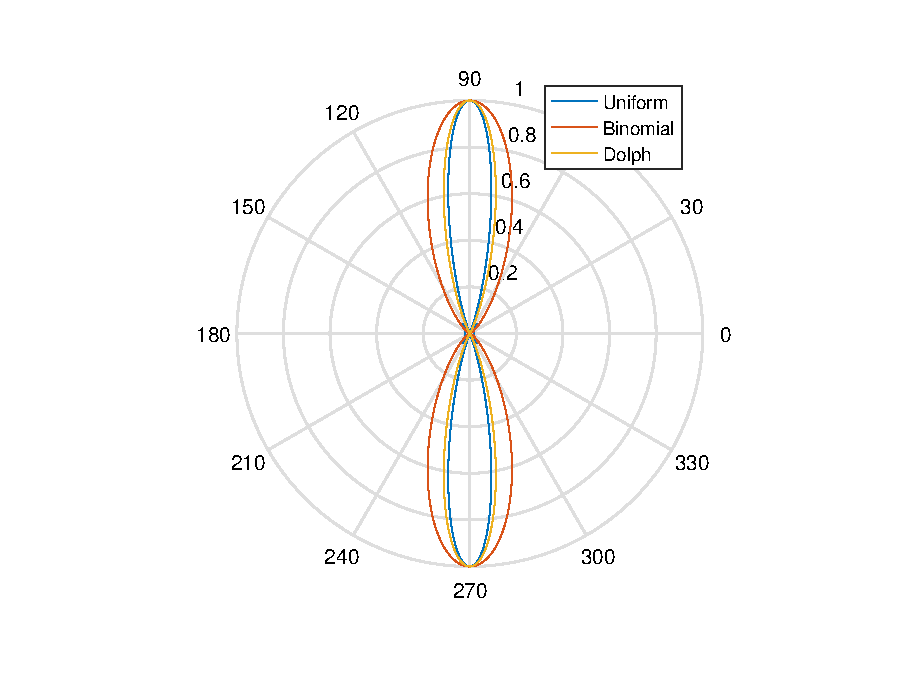
\includegraphics[height=5.5cm,width=7.5cm]{TenEle_without_EF.eps}
		\caption{Pattern without EF}\label{fig:10elenoEF}
	\end{minipage}%
	\hfill
	\begin{minipage}[t]{0.5\linewidth}
		\centering
		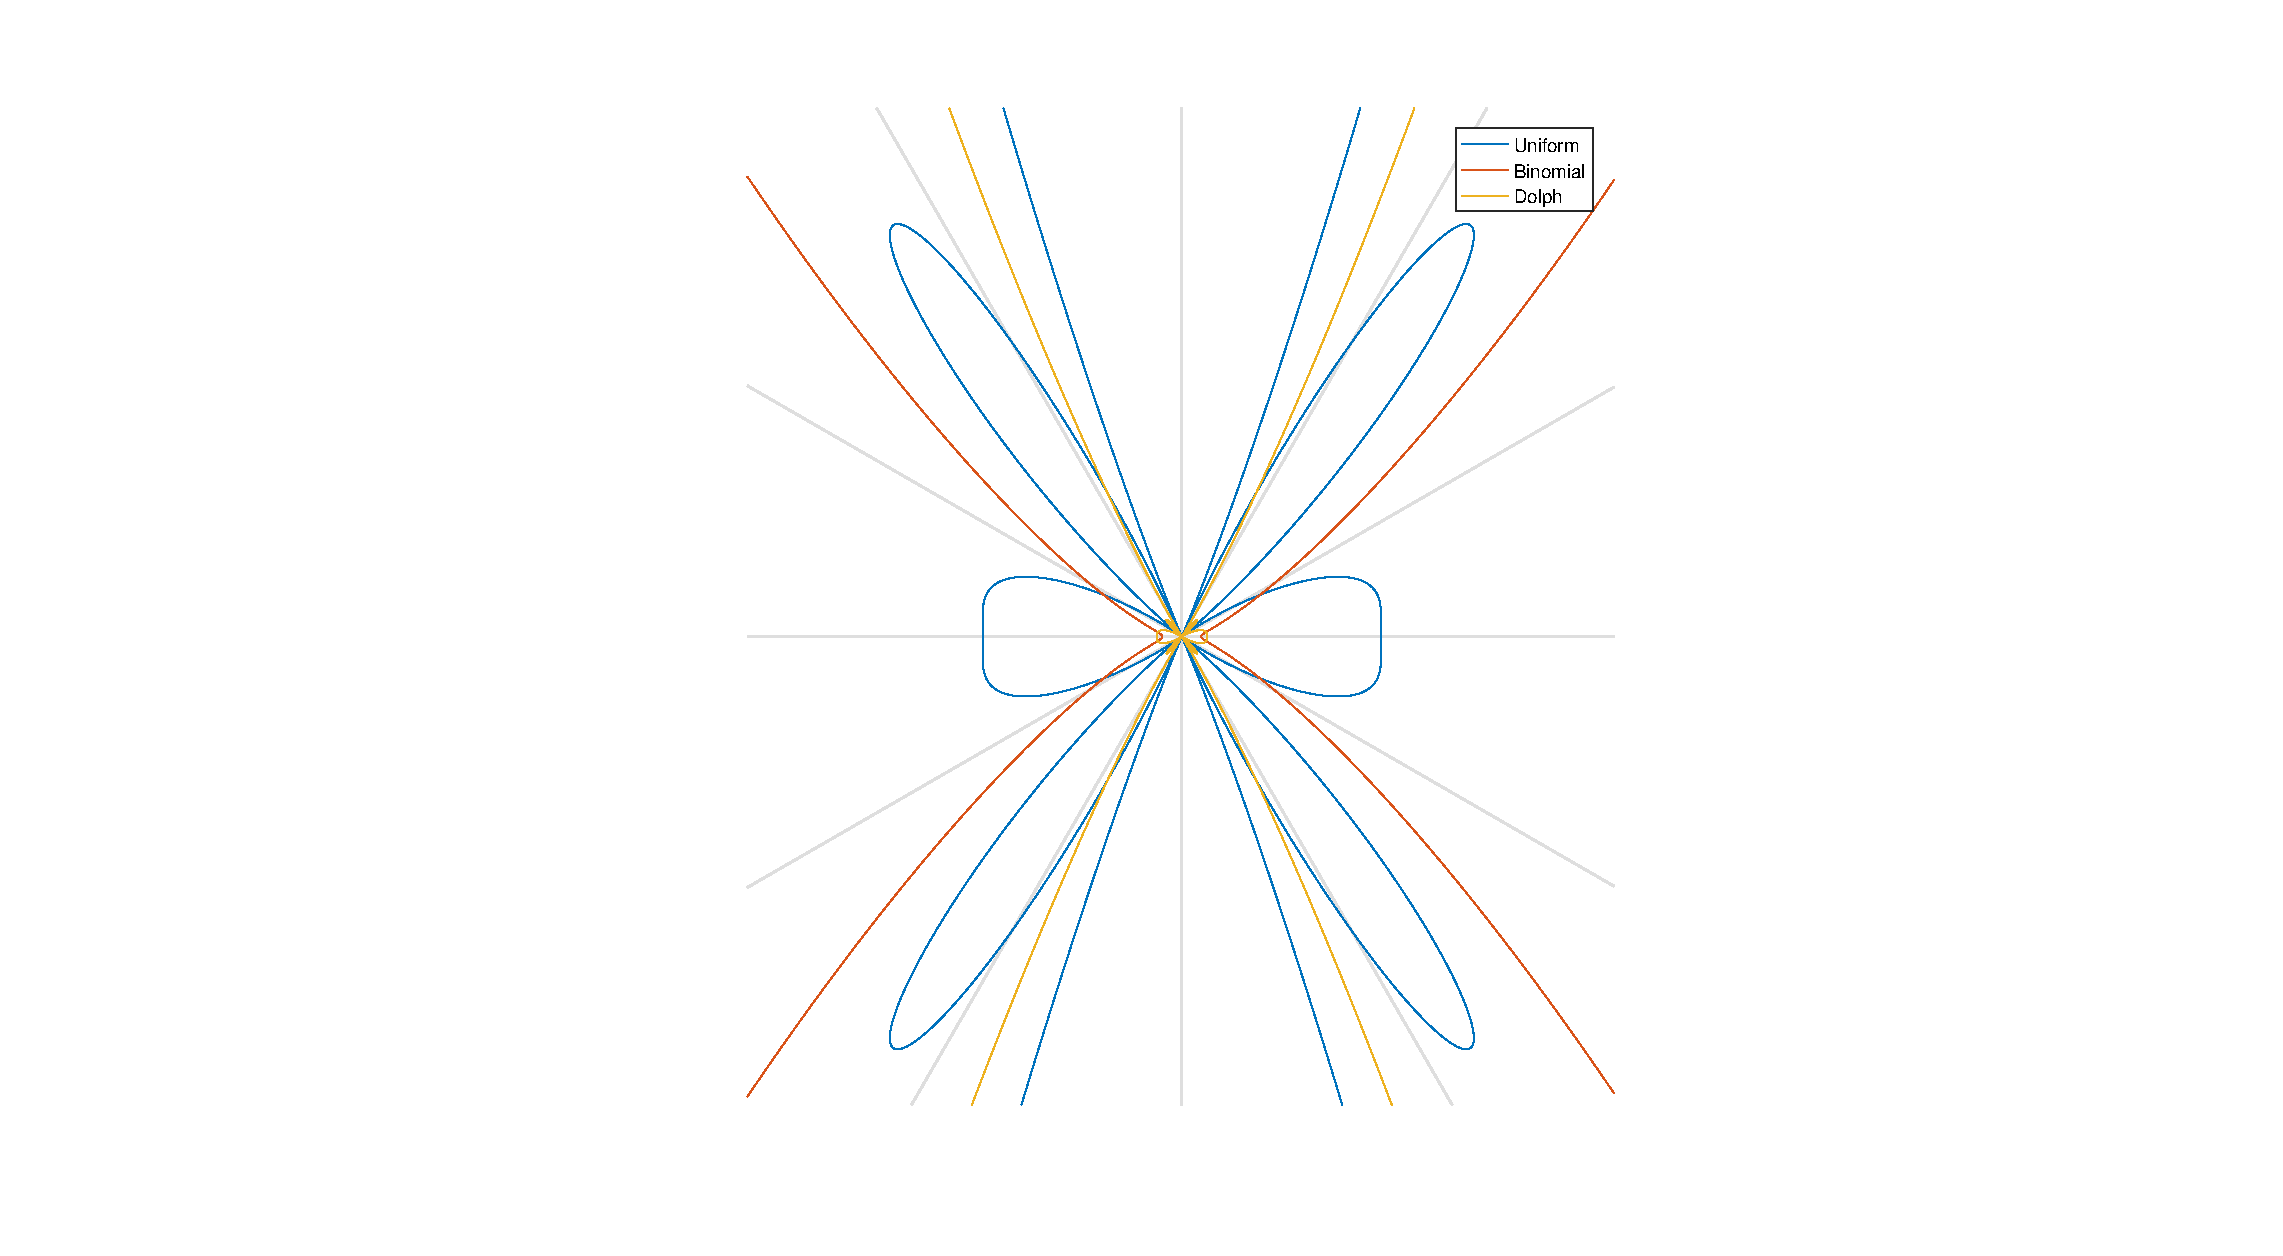
\includegraphics[height=5.5cm,width=7.5cm]{TenEle_without_EF_fangda.eps}
		\caption{放大图}\label{fig:10elenoEF_fangda}
		
	\end{minipage}
\end{figure}


\subsubsection{选做:与经验公式比较}


\subsubsection{选做:考虑单元因子的边射阵方向图}
\begin{figure}[!ht]
	\begin{minipage}[t]{0.35\linewidth}
		\centering
		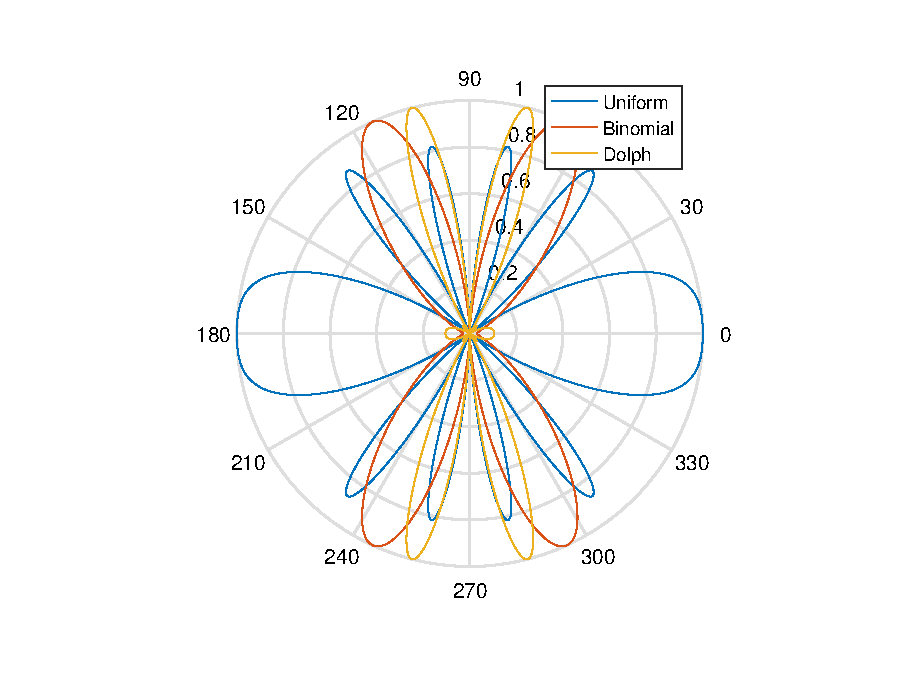
\includegraphics[height=5.5cm,width=7.5cm]{TenEle_with_EF.eps}
		\caption{Pattern with EF}
	\end{minipage}%
	\hfill
	\begin{minipage}[t]{0.5\linewidth}
		\centering
		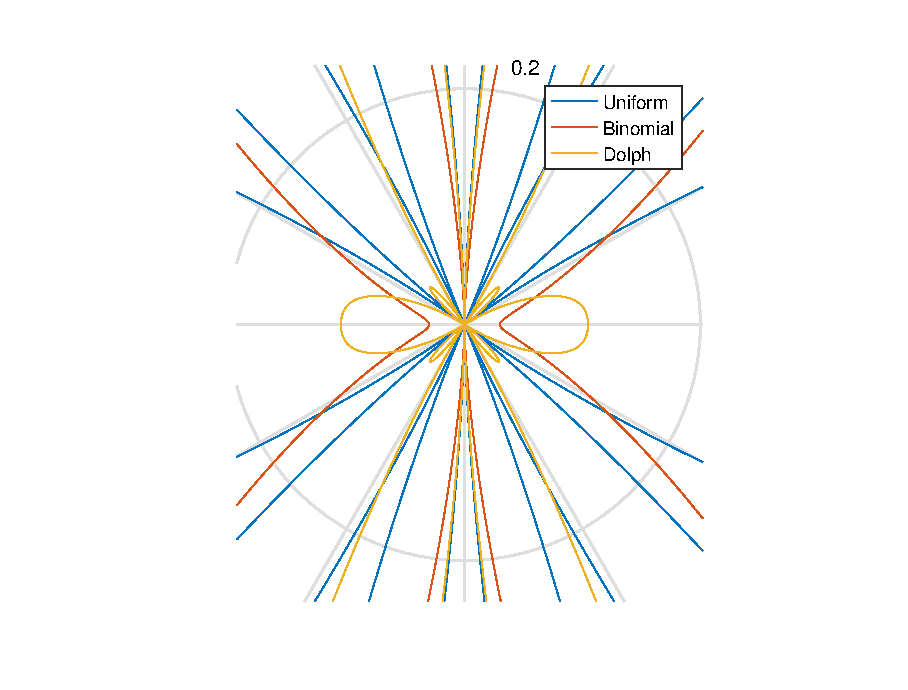
\includegraphics[height=5.5cm,width=7.5cm]{TenEle_with_EF_fangda.eps}
		\caption{放大图}
		
	\end{minipage}\label{fig:10eleEF}
\end{figure}

\subsection{程序}
\noindent \textbf{主程序}
\begin{lstlisting}[language={matlab},keywordstyle=\color{blue!70},commentstyle=\color{red!50!green!50!blue!50},frame=shadowbox, rulesepcolor=\color{red!20!green!20!blue!20}] 


\end{lstlisting}